%----------------------------------------------------------------------------------------
%	PACKAGES AND OTHER DOCUMENT CONFIGURATIONS
%----------------------------------------------------------------------------------------

\documentclass[12pt]{article}
\usepackage{polski}
\usepackage[polish]{babel}
\usepackage[utf8]{inputenc}
\usepackage{datetime}
\usepackage{graphicx}
\usepackage{tikz}
\usepackage{amsmath}
\usepackage{multirow}
\usepackage{tabularx}
\usepackage{geometry}
\usepackage{subcaption}
\usepackage{epstopdf}

\geometry{
 	a4paper, 
 	left    = 20mm,
 	right	  = 20mm,
 	top     = 20mm,
 	bottom  = 20mm,
}
 
%----------------------------------------------------------------------------------------
 
%----------------------------------------------------------------------------------------
% DATES
%----------------------------------------------------------------------------------------

\renewcommand{\dateseparator}{.}
\newdate{exercise_date}{15}{12}{2016}



% dodatkowe typy kolumn tabel

% flush left fixed width:
\newcolumntype{L}[1]{>{\raggedright\arraybackslash}p{#1}}

% center fixed width:
\newcolumntype{C}[1]{>{\centering\arraybackslash}p{#1}}

% flush right fixed width:
\newcolumntype{R}[1]{>{\raggedleft\arraybackslash}p{#1}}

%----------------------------------------------------------------------------------------

%----------------------------------------------------------------------------------------
% TIKZ PACKAGES
%----------------------------------------------------------------------------------------

\usetikzlibrary{arrows}

%----------------------------------------------------------------------------------------

\begin{document}
 
\begin{titlepage}

\newcommand{\HRule}{\rule{\linewidth}{0.5mm}}
% Defines a new command for the horizontal lines, change thickness here

\center
% Center everything on the page
 
%----------------------------------------------------------------------------------------
%	LOGO SECTION
%----------------------------------------------------------------------------------------


\includegraphics[width=6cm]{./img/logo.png}\\[1cm]
% Include a department/university logo - this will require the graphicx package
 
%----------------------------------------------------------------------------------------
 
%----------------------------------------------------------------------------------------
%	HEADING SECTIONS
%----------------------------------------------------------------------------------------

\textsc{\LARGE Akademia Górniczo-Hutnicza \\[0.2cm]
im. Stanisława Staszica w Krakowie}\\[1.5cm]
% Name of your university/college

\textsc{\Large Elektroniczne systemy diagnostyki medycznej i terapii}\\[0.5cm]
% Major heading such as course name

%----------------------------------------------------------------------------------------
%	TITLE SECTION
%----------------------------------------------------------------------------------------

\HRule \\[0.5cm]
{ \huge \bfseries Odszumianie sygnału metodą nielokalnych średnich}\\[0.3cm]
% Title of your document
\HRule \\[1.5cm]

\flushright
\Large \emph{Autorzy:}\\
Tomasz \textsc{Gawlik}\\[0.1cm]  % Your name
Tomasz \textsc{Kańka}\\[3cm]        % Your name
% Authors

%----------------------------------------------------------------------------------------
%	DATE SECTION
%----------------------------------------------------------------------------------------
% Data wykonania ćwiczenia: \\
%{\large \displaydate{exercise_date}}\\[1cm]


\vfill % Fill the rest of the page with whitespace

\end{titlepage}
\tableofcontents
\section{Wstęp}

Niezwykle istotnym z punktu widzenia analizy sygnału EKG jest oddzielenie rzeczywistego sygnału od szumu, który nakłada się na sygnał podczas badania. Jedną z technik stosowanych do odszumowania sygnału ekg jest jest filtr nielokalnych średnich (ang. nonlocal means NLM). Metoda polega na uśrednieniu podobnych fragmentów przebiegu, które powtarzają się na przestrzeni całego badania. Można zaryzykować stwierdzenie że sygnał EKG jest okresowy więc powyższa metoda powinna wiernie odwzorować realny przebieg. 
\section{Algorytm}
\label{ch:algorytm}
Celem algorytmu jest odtworzenia poprawnego sygnału $u$ z zarejestrowanego przebiegu $v = u + g$, gdzie $g$ jest addytywnym szumem. Dla podanej próbki sygnału $s$ estymata  $\hat{u}\left ( s \right )$ stanowi sumę ważoną innych próbek $t$ które zawierają się w sąsiedztwie $N(s)$ 


\begin{equation}
\label{eq:jeden}
\hat{u}\left(s\right)= \frac{1}{Z(s)} \sum_{t\in N(s)} w(s,t)v(t)
\end{equation}

gdzie $Z(s) = \sum_{t} w(s,t)$, a waga dla próbki wynosi $w$:

\begin{equation}
\label{eq:dwa}
w(s,t)= \textup{exp} \left (  -\frac{\sum_{\delta \in \Delta }{(v(s+\delta)-v(t+\delta))^{2}}}{2L_{\Delta}\lambda^{2}}\right ) \equiv \textup{exp} \left ( -\frac{d^{2}(s,t)}{2L_{\Delta}\lambda^{2}}\right )
\end{equation}

W równaniu (\ref{eq:dwa}) $\lambda$ jest parametrem opisującym pasmo, podczas gdy $\Delta$ reprezentuje lokalny fragment próbek wokół punktu $s$, zawierający $L_{\Delta}$ próbek. Okolice punktu $t$ są analizowane wycinkiem o tym samym kształcie.

Należy zwrócić uwagę, że $w(s,s)=1$. Stosując metodą NLM dla zaszumionych obrazów, często zakłada się, że:
\begin{equation}
\label{eq:trzy}
w(s,s) = \max_{t\in N(s),t\neq s}w(s,t)
\end{equation}
W przypadku odszumiania sygnału EKG, stosując powyższą korektę dochodzi do nadmiernego gładzenia niektórych zespołów QRS, co widoczne jest na rysunku \ref{rys:rzekomapoprawa}. Pozostano więc przy oryginalnej wadze  $w(s,s)=1$.
\begin{figure}[!htb]
	\begin{center}
		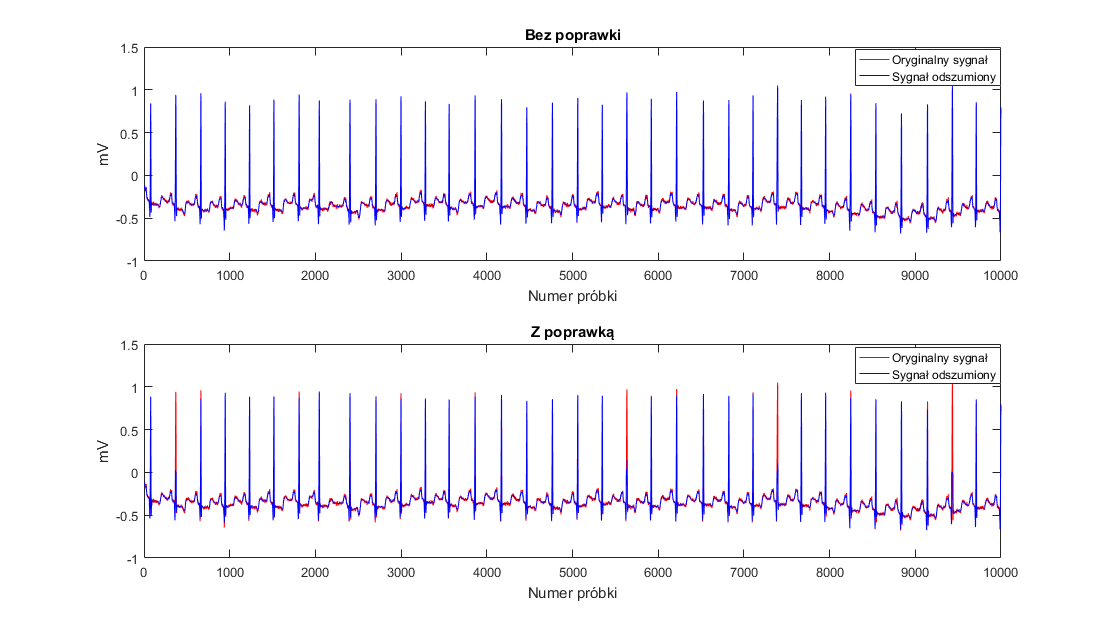
\includegraphics[width=15cm,clip]
		{img/rzekomapoprawa.png}
	\end{center}
	\caption{Sprawdzenie wprowadzenia korekty opisanej wzorem \ref{eq:trzy}. Wprowadzona poprawka tak naprawdę pogarsza estymatę oryginalnego sygnału EKG.}
	\label{rys:rzekomapoprawa}
\end{figure}

Cechą odróżniającą metodę NLM są wagi $w(s,t)$ które zależą od podobieństwa między fragmentami, a nie odległością między punktami $s$ i $t$. Uśrednianie podobnych fragmentów pozwala na znacznie lepsze  zachowanie zboczy sygnału niż inne typowe filtry (np. Gaussowski, dolnoprzepustowy).  Biorąc pod uwagę że podobieństwo między fragmentami jest widoczne na całym przebiegu, może on być uznany za sąsiedztwo badanego fragmentu. Taki zabieg powoduje że proces jest całkowicie nielokalny.\cite{tracey2012nonlocal}


\section{Dobór parametrów}
\label{ch:parametry}

Przy implementacji filtru NLM pojawia się problem doboru parametrów algorytmu. Pierwszym parametrem jest $P$ określąjący maksymalną odległość próbki należącej do $\Delta$ od punktu $s$, a więc $L_\Delta=2P+1$. Dla sygnałów EKG odpowiednim wyborem dla $P$ jest liczba w okolicach połowy długości zespołu QRS.

\begin{figure}[!htb]
	\begin{center}
		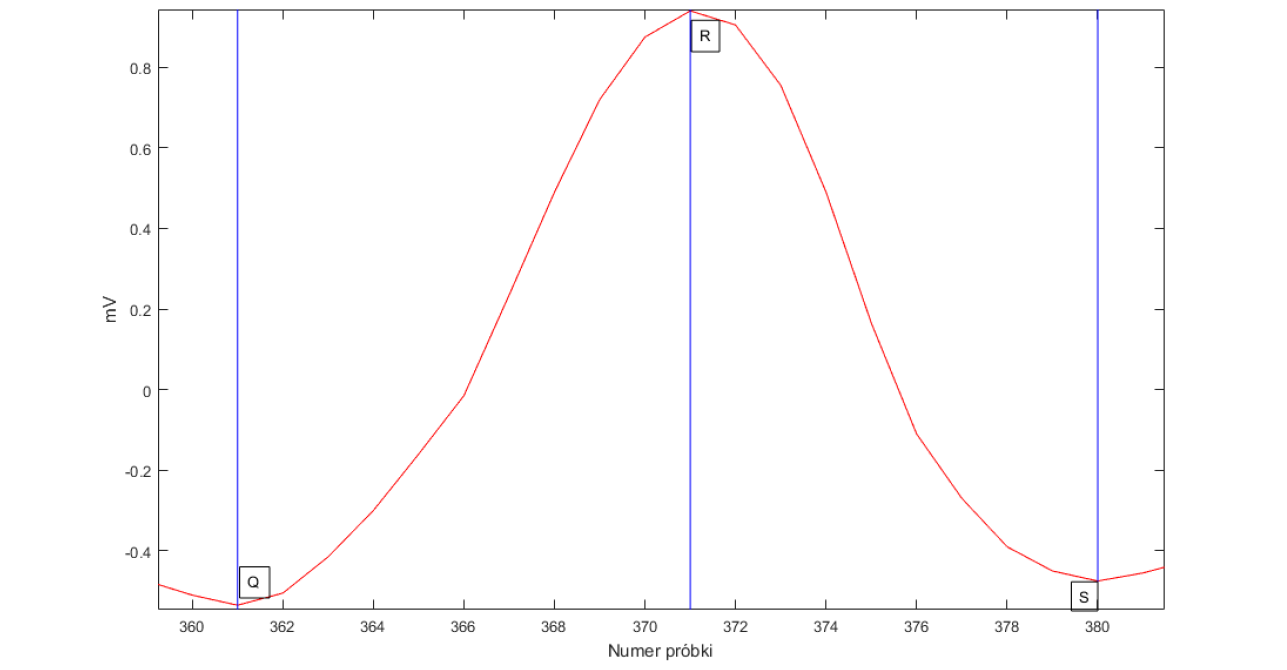
\includegraphics[width=15cm,clip]
		{img/qrs.png}
	\end{center}
	\caption{Fragment sygnału EKG zawierający zespół QRS. Sygnał pochodzi z Physionet MIT-BIH arrythymia database i jest oznaczony numerem 100.\cite{mitbih} }
	\label{rys:qrs}
\end{figure}
Z rysunku \ref{rys:qrs}. wynika, że odpowiednią wartością będzie $P=10$ próbek.

Parametr M reprezentuje połowę rozmiaru otoczenia $N(s)$ (czyli $|N(s)| = 2M+1$). Zapewnia on ,,mniej lokalne''  przeszukiwanie sygnału. Zakładając, że sygnał EKG jest praktycznie okresowy, im więcej ,,okresów'' zostanie uwzględnionych w obliczaniu estymaty $\hat{u}(s)$ tym lepsze wyniky powinno się uzyskać. Jednakże zbytnie zwiększenie obszaru poszukiwań powoduje dłuższe obliczenia. Przyjęto, że $M=2000$, a co za tym idzie, obszar poszukiwań obejmuje około 15 ,,okresów'' sygnału ECG.

Ostatnim, ale naistotniejszym parametrem jest pasmo $\lambda$, który odpowiada za wygładzenie estymaty zaszumionego sygnału EKG. Zbyt mała $\lambda$ powoduje złe dopasowanie wag przy uśrednianiu, zbyt duża wartość tego parametru skutkuje w traktowaniu niepodobnych do siebie fragmentów sygnału jako podobnych. Parametr ten zależy od wariancji $\sigma^2$ szumu i można przyjąć, że $\lambda=\frac{6}{10}\sigma$. Parametr ten został dobrany doświadczalnie, na bazie analizy zaszumionych przebiegów, wobec czego przyjęto, że $\sigma^2=0,0004$.\cite{tracey2012nonlocal}.
\section{Prototyp programu}

Prototyp programu zrealizowano w środowisku Matlab. Tę decyzję podjęto ze względu na łatwość implementacji algorytmu w tym środowisku, znajomość autorów projektu języka Matlab oraz szybką możliwość wizualizacji osiągniętych wyników.

Dla ujednolicenia oznaczeń przyjmijmy, że $ n $ oznaczna liczbę próbek sygnału wejściowego. Prototyp został podzielony na dwie zasadnicze części:

\begin{enumerate}
	\item Wczytanie danych pomiarowych, wywołanie funkcji zawierającej implementację metody nielokalnych średnich oraz wyrysowanie wyników.
	\item Funkcja odszumiająca sygnał wejściowy metodą NLM
\end{enumerate}

\subsection{Implementacja metody NLM}
\label{ch:implementacja}
Implementacja funkcji odszumiającej odbyła się zgodnie z opisem w rozdziale \ref{ch:algorytm}. 

Zasadniczo, składa się ona z 3 zagnieżdżonych w sobie pętli. Najbardziej zewnętrzna z nich ma za zadanie przejść przez wszystkie próbki sygnału wejściowego $ v(s) $ oraz uzyskać $ \hat{u}(s) $ zgodnie z \eqref{eq:jeden}.

Środkowa pętla odpowiada za wyliczenie \eqref{eq:dwa} przy ustalonym $ s $ dla każdego $ t\in N(s) $. Uzyskany wynik dla każdej iteracji dodawany jest do zmiennej \texttt{Z} oraz mnożony przez $ v(t) $ i dodawany do \texttt{Mult}, w celu wyznaczenia odpowiednio $ Z(s) $ oraz sumy z równania \eqref{eq:jeden}.

Wewnętrzna pętla ma za zadanie wyznaczyć $ d^{2}(s,t) $ pomiędzy próbkami $ s $ i $ t $ zgodnie z \eqref{eq:dwa}. 

\subsection{Wizualizacja uzyskanych wyników}
Główny program ma za zadanie wczytać dane wejściowe, przekazać je do funkcji odszumiającej opisanej w \ref{ch:implementacja} wraz z parametrami, których dobór odbył się zgodnie z rodziałem  \ref{ch:parametry}. Po otrzymaniu wyniku filtracji program główny przystępuje do wizualizacji uzyskanych rezultatów. Odbywa się to w formie wykresu porównującego dane oryginalne z danymi odszumionymi.

Warto zaznaczyć, że dla próbek $ s $ o numerach od $ 1 $ do $ P $ oraz od $ n-P+1 $ do $ n $ lokalny fragment wokół $ s $ jest mniejszy niż dla pozostałych próbek. Postanowiono dla nich jako estymatę przyjąć sygnał wejściowy. Takie podejście nie wpływa w sposób zauważalny na rezultat, gdyż $ P\ll n $.
\section{Implementacja algorytmu w C++}

Prototyp zrealizowany w środowisku Matlab pozwolił na bardzo szybką implementację algorytmu w C++. Miała ona na celu przyspieszenie dokonywanych obliczeń.

Program napisany w C++ ma strukturę jednoplikową i w samym działaniu odbiega od prototypu tylko pod kątem braku wizualizacji wyników. W zamian, rezultat zapisywany jest do pliku tekstowego.

Kompilacja programu została przetestowana pod kompilatorem GCC 5.3.0 na systemie operacyjnym Microsoft Windows 10. Ważną kwestią okazało się dodanie flagi automatycznej optymalizacji \texttt{-Ofast} podczas wykonywania polecenia \texttt{g++ main.cpp}, w przeciwnym wypadku program w C++ wykonywał się znacznie dłużej niż prototyp w Matlabie. 

Podczas uruchamiania programu istnieje możliwość przekazania argumentów z poziomu wiersza poleceń. Parametry te to kolejno nazwa pliku wejściowego, nazwa pliku wyjściowego, parametr $ P $, parametr $ M $ oraz parametr $ \lambda $. W przypadku nie podania argumentów przyjmują one wartości domyślne:

\begin{table}[!htb]
	\centering
	\caption{Domyślne wartości argumentów funkcji \texttt{main}. Parametry liczbowe zostały przyjęte zgodnie z rodziałem \ref{ch:parametry}. }
	\begin{tabular}{|c|l|l|}
		\hline
		Argument & Wartość domyślna \\
		\hline
		Nazwa pliku wejściowego & \texttt{input} \\
		\hline
		Nazwa pliku wyjściowego & \texttt{output} \\
		\hline
		$P$ & $10$ \\
		\hline
		$M$ & $2000$ \\
		\hline
		$\lambda$ & $0.012$ \\
		\hline
	\end{tabular}
	\label{tab:tabela1}
\end{table}

Do przechowywania danych wejściowych oraz sygnału odszumionego wykorzystano darmową bibliotekę Eigen.
\section{Porównanie implementacji w Matlabie oraz w C++}

Istotną sprawą jest sprawdzenie, czy występują znaczące różnice między implementacją w Matlabie oraz w C++. W celu porównania sprawdzono rozbieżności pomiędzy implementacjami (wizualnie) oraz czas obliczeń.

\subsection{Rozbieżności między implementacjami}

W celu porównania rezultatów uzyskanych w Matlabie oraz w C++ dokonano próby odszumienia sygnału oznaczonego numerem 100 (pierwsze 100000 próbek) pochodzącego z Physionet MIT-BIH arrythymia database\cite{mitbih} obydwoma programami. Parametry algorytmu w obu przypadkach są takie same (domyślne). Następnie zestawiono wyniki na wspólnym wykresie.

\begin{figure}[!htb]
	\begin{center}
		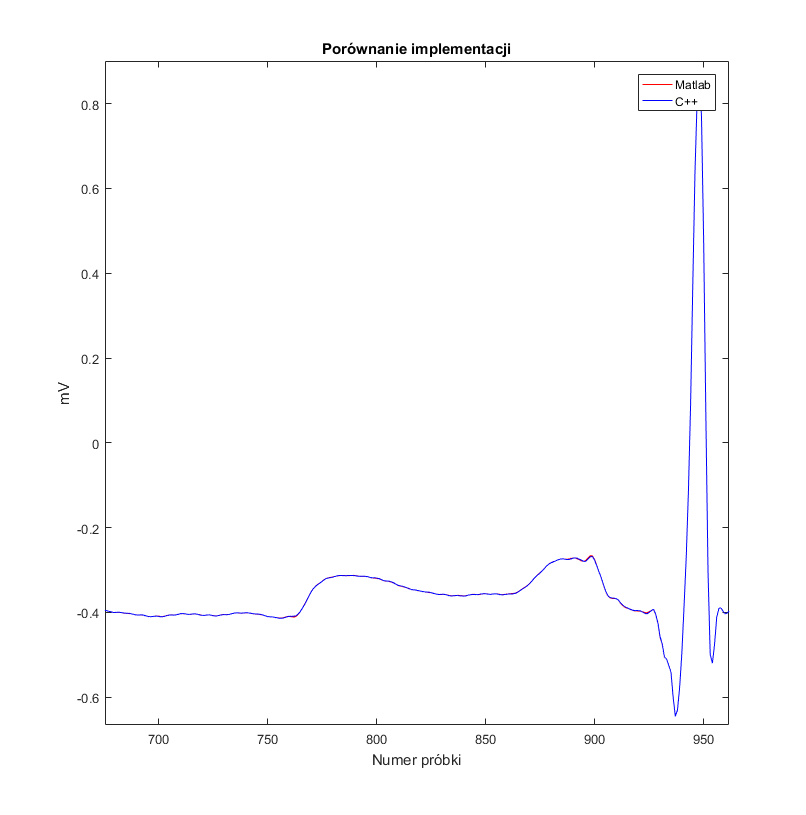
\includegraphics[width=15cm,clip]
		{img/porownanie.png}
	\end{center}
	\caption{Porównanie obydwu implementacji. Wykres został przybliżony na jeden pseudookres, ze względu na brak czytelności wykresu. }
	\label{rys:porownanie}
\end{figure}

Rysunek \ref{rys:porownanie} dowodzi, że implementacja w C++ i w Matlabie dają podobne rezultaty. Nieznaczne różnice mogą wynikać z różnic pomiędzy precyzjami typów \texttt{double} w obu językach.

\subsection{Czasowe porównanie implementacji}

Obydwie implementacje dają podobne rezultaty. Można zatem porównać czas wykonywania obydwu programów. Programy zostały uruchomione na komputerze z procesorem Intel i7 4790.
\begin{table}[!htb]
	\centering
	\caption{Tabela porównująca czasy wykonania programu.}
	\begin{tabular}{|c|l|l|}
		\hline
		Język & Czas [$\mathrm{s}$] \\
		\hline
		Matlab & 96,958 \\
		\hline
		C++ & 22,937 \\
		\hline
	\end{tabular}
	\label{tab:tabela2}
\end{table}

Niekwestionowanym zwycięzcą jest C++. Warto jednak zauważyć, że bez flagi \texttt{-Ofast} program w C++ wykonuje się znacznie dłużej (dla takiego samego zestawu danych - kilkanaście minut).

Czas wykonywania programu może wydawać się bardzo długi, jednak jest on związany z dużą złożonością obliczeniową. Wykonywane są 3 zagnieżdżone w sobie pętle. Dla parametrów domyślnych instrukcje z wewnętrznej pętli programu wykonują się około $(n-2P-1)\cdot(2M+1)\cdot(2P+1)$ razy, co dla domyślnych parametrów i serii 100 tysięcy próbek daje około 8 miliardów iteracji.
\section{Wnioski}

Projekt miał na celu zapoznanie się z metodą nielokalnych średnich w odszumianiu sygnału EKG. Algorytm NLM jest wykorzystywany przede wszystkim w odszumianiu obrazów, ale, jak widać, jego wersja ,,jednowymiarowa'' jest również skuteczna w odszumianiu sygnałów biomedycznych.

Warto zauważyć, że metoda praktycznie nie ingeruje w okolicach załamki Q. Jest to związane z tym, że różnice wartości sygnału między dowolnymi próbkami $s$ i $t$ w obrębie załamki Q są duże, a co za tym idzie, wagi w tym punkcie są małe.

Algorytm jest stosunkowo wolny. W celu przyspieszenia działania można zastosować dwie zmiany w działaniu:
\begin{enumerate}
	\item Zrównoleglenie wyliczeń i wykorzystanie GPU
	\item Wykorzystanie algorytmu zaproponowanego w artykule ,,\textit{Fast nonlocal filtering applied to electron cryomicroscopy}''\cite{DarbonCCOJ08}
\end{enumerate} 

W projekcie użyto dwóch implementacji tego samego algorytmu. Prototyp programu pozwala na szybką implementację wybranego algorytmu w języku niekompilowanym. Służy on do testowania poprawności implementacji i ma na celu ułatwienie napisania programu wyjściowego. Sam program ma za zadanie przyspieszyć obliczenia. Taka konwencja znacznie przyspiesza proces tworzenia oprogramowania.

\bibliographystyle{plain}
\bibliography{reference}

\end{document}